\documentclass{beamer}
\usepackage[latin1]{inputenc}
\usepackage{tabularx}
\usepackage{graphicx}
\usepackage{epstopdf}

\usetheme{Antibes}
\title[CryptoSMS]{CryptoSMS\\Text message encryption for Android}
\author{David Brazdil}
\institute{University of Cambridge}
\date{September 15, 2011}

\begin{document}

\begin{frame}
\titlepage
\end{frame}



\begin{frame}{Data format for SMS}
\newcolumntype{L}{>{\raggedright\arraybackslash}X}%

First message: \\
\begin{tabularx}{\textwidth}{ |l|l|l|L| }
  \hline
  type    & id      & count   & data \\
  2 bits  & 14 bits & 1 byte  & 130 bytes  \\
  \hline
\end{tabularx} \newline
\\
Other parts: \\
\begin{tabularx}{\textwidth}{ |l|l|l|L| }
  \hline
  type    & id      & index   & data \\
  2 bits  & 14 bits & 1 byte  & 130 bytes  \\
  \hline
\end{tabularx}

\end{frame}



\begin{frame}{Secure storage file}
\begin{figure}
\centering
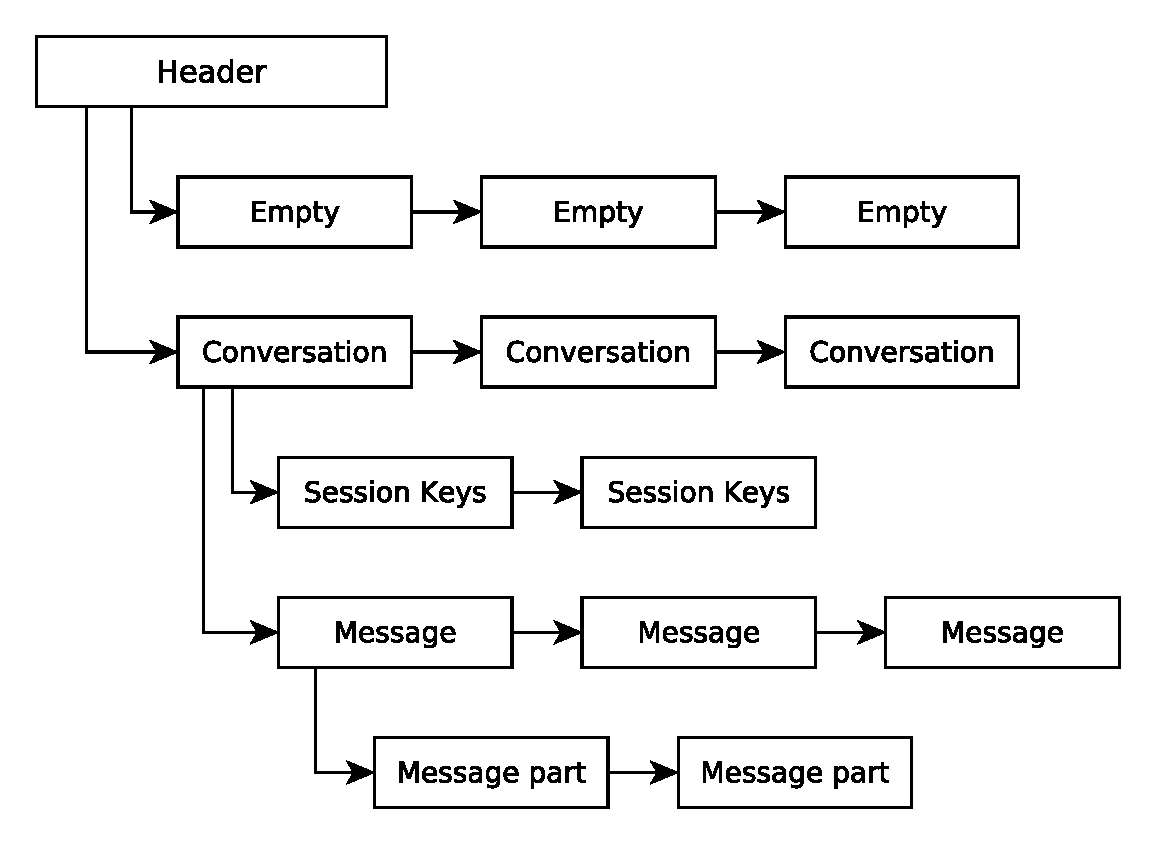
\includegraphics[width=0.7\textwidth]{storage_file}
\end{figure}
\end{frame}

\end{document}